\documentclass [9 pt]{article}
\usepackage[margin = 1in]{geometry}
\usepackage{amsfonts}
\usepackage{amsthm}
\usepackage{bbm}
 \usepackage{amsmath}
\usepackage[utf8]{inputenc}
\usepackage{graphicx}
\usepackage{ wasysym }
\usepackage{enumerate}
\usepackage{color}
\usepackage{graphicx}
\graphicspath{ {./images/} }
\usepackage{tikz}
\usepackage{booktabs}

\theoremstyle{definition}
\newtheorem{problem}{Problem}
\newtheorem{theorem}{Theorem}
\newtheorem*{corollary}{Corollary}
\newtheorem{proposition}[theorem]{Proposition}
\newtheorem{lemma}[theorem]{Lemma}
\newtheorem{conjecture}[theorem]{Conjecture}

\newtheorem{definition}[theorem]{Definition}
\newtheorem{remark}[theorem]{Remark}
\newtheorem{example}[theorem]{Example}


\usepackage{fancyhdr}
\pagestyle{fancy}
\lhead{Yuhao Wu \quad 260711365} 
\rhead{\bfseries COMP 330 Assignment 2}
\cfoot{\thepage}
\renewcommand{\headrulewidth}{0.4pt}
\renewcommand{\footrulewidth}{0.4pt}



\setlength{\parindent}{0pt}

\begin{document}

\title{COMP 330 Assignment 3}
\date{2018-10-6}
\author{Name: Yuhao Wu\\
ID Number: 260711365
}
\maketitle


\section*{Question 1:}
Are the following statements true or false? Prove your answer in each case. We have some fixed alphabet $\Sigma$ with at least two letters. In the following $A$ and $B$ stand for languages, i.e. subsets of $\Sigma^*$.
\begin{itemize}
	\item If $A$ is regular and $A \subseteq B$ then $B$ must be regular. 
	\item If $A$ and $AB$ are both regular then $B$ must be regular. 
	\item  If $\{A_i\ |\ i   \in \mathbb{N}  \} $ is an infinite family of regular sets then $ \bigcup_{i = 1}^{\infty} A_i$ is regular. 
	\item  If $A$ is not regular it cannot have a regular subset.
\end{itemize}


\subsection*{(a):}
\textbf{FALSE}\\
\newline
We take $A = \{ \varepsilon \}$, $B = \{\  a^n \ b^n | n \geq 0\  \}$\\
\newline
Then we have $A$ is regular \quad $A \subseteq B \quad B $ is not regular.

\subsection*{(b):}
\textbf{FALSE:}\\
\\
Suppose that our alphabet $\Sigma$ is $\{\ a, b \ \}$.\\
Then I choose $A = a^*$\quad \quad $B = \{ a^i\ |\ i\text{  is a prime number } \}$,\\
 then we have $B\subseteq A$. Thus, we can say that $AB = a^*$, which is regular.
 And $A$ is regular as well.\\
 While as we have seen in class, $B = \{ a^i\ |\ i\text{  is a prime number } \}$ is not regular.\\
 Thus, we can say that If $A$ and $AB$ are both regular then $B$ can be non-regular. 


\subsection*{(c):}
\textbf{FALSE:} \\
\newline
Suppose that $A_i$ is an infinite family of regular languages. Then this statement cannot be true.\\
 Because every language is the union of some set of regular languages. Let $L$ be an arbitrary language whose words are $w_1, w_2, w_3, \ldots $. \\
 Let $A_i$ be the set of singleton languages $\{ \{w_1\}, \{w_2\}, \{w_3\}, \ldots  \}$, such that $w_i \in L$. The number of elements of $A_i$ is equal to the cardinality of $L$.\\
  Each individual element of $A_i$ is a language that contains a single string, so for each element of $A_i$ it is a regular set containing only one word.\\
   $L = \bigcup_{i = 1}^{\infty}A_i$. As not all languages are regular, it must exist  case that $\bigcup_{i = 1}^{\infty}A_i$ is not to be regular. 
\subsection*{(d):}

$$\text{ $A$ is not regular } \implies \text{ A cannot have a regular subset } $$
$$ \neg \bigg(\text{ A cannot have a regular subset } \bigg)  \implies \neg \bigg( \text{ $A$ is not regular } \bigg) $$
$$ \text{ A  have a regular subset }  \implies\text{ $A$ is regular } $$
which is the same as Question.(a):\\
\\
We take $A = \{ \varepsilon \}$, $B = \{\  a^n \ b^n | n \geq 0\  \}$\\
\newline
Then we have $A$ is regular \quad $A \subseteq B \quad B $ is not regular.























\newpage
\section*{Question 2:}
Show that the following language is not regular using the pumping lemma. 
$$ L = \{a^n b a^{2n}|n > 0 \}$$
\\
\newline\newline


\begin{itemize}
	\item Demon picks a random positive integer $p$\\
	\item I pick the string $w = a^{p}\ b\ a^{2p}$. Obviously, we have $|w| \geq p$ \\
	\item Demon is now need to choose $x, y, z$ such that $xyz = w$.\\ As $|x\ y| \leq p$ and $|y| > 0$, Demon is forced to pick $y$ to consist of a nonempty string that consists of "a" only\\
	We say that $y = a^{k}\quad 0 < k \leq p$\\
	\item Now I choose $i = 2$. The new string is $a^{p+k}\ b\ a^{2p}$ which is not in the language as 
	 $$ \dfrac{p + k}{2p} = \dfrac{1}{2} + \dfrac{k}{2p} > \dfrac{1}{2} $$
\end{itemize}






















\newpage
\section*{Question 3:}
Show that the language
$$F = \{a^i\ b^j\ c^k \ | \ i,j,k\geq 0 \text{ and if } i = 1 \text{ then }  j = k  \}$$
is not regular. Show, however, that it satisfies the statement of the pumping lemma as I proved it in class, i.e. there is a $p$ such that all three conditions for the pumping lemma are met. Explain why this does not contradict the pumping lemma.\\
\newline
\newline
\textbf{Show "F" is not regular:}\\
Suppose $F$ is regular, then I will choose another regular language $L$. As we have seen in class, if $F, L$ is regular, then $F \cap L$ is regular.\\
I choose $L$ to be $\big( a\ b^* \ c^* \big)$. Obviously, $L$ is regular.\\
As the word in $L$ starts with exactly only one $a$, if it is also in $F$, we must have $j = k$, which means $$F \cap L = \{ a\ b^j\ c^j \ | \ j\geq 0 \}$$
As we have seen in class, $F \cap L$ is not regular, which means $F$ is not regular.\\
\newline\newline\newline
\textbf{Show "F" satisfies the statement of the Pumping Lemma}\\
\begin{itemize}
	\item I choose a number $p,\ p \in \mathbb{N},\ p > 0 $
	\item Demon chooses a random word $w$ in $F$, such that $|w| \geq p$
	\item I choose $x, y, z$ and $w = xyz$, such that $|xy| \leq p\ \&\ |y| >0$
	\item Demon randomly choose number $n \in \mathbb{N}$, we need to show if $x y^n z$ is also in $F$
\end{itemize}
I choose $p = 2$\\\newline
\textbf{[1]:}Consider Demon chooses word $w =  b^{j}c^{k}$, which means $i = 0$ Then choose $x= \varepsilon $ and 
\begin{itemize}
	\item  $y=b$ if $j \neq 0$
	\item  $y=c$ if $j = 0 $\quad which means $w$ contains $c$ only.
\end{itemize} 
If $y=b$, then $z = b^{j-1} c^{k}$, and $xy^nz = b^n b^{j-1} c^{k}$, which is clearly in $F$ for any $n$.\\
\newline
If $y=c$, then $z =  c^{k - 1}$, and $xy^nz = c^n c^{k-1}$, which is clearly in $F$ for any $n$.\\
\newline
\newline
\textbf{[2]:} Consider Demon chooses word $w = a b^{j}c^{j}$, which means $i = 1$ Then choose $x= \varepsilon ,y = a, z = b^{j}c^{j} $\\\\
We will get the string in the form of $$x\ y^n\ z = a^n\ b^j\ c^j$$\\
As the number of b's is the same as the number of a's, regardless of whether pumping up or pumping down, $xy^nz $ will always be in $F$\\
\newpage
\textbf{[3]:} Consider Demon chooses word $w = a^2 b^{j}c^{k}$, which means $i = 2$ Then choose $x= \varepsilon ,y = a^2, z = b^{j}c^{j} $\\
\newline
We will get the string in the form of $$x\ y^{n}\ z = a^{2n}\ b^j\ c^k$$\\
Thus, regardless of pumping up or pumping down, we will never have the case with only one $a$, so we don't need to worry about whether $j$ equals $k$ or not.\\
Thus, $xy^nz $ will always be in $F$.\\
\newline\newline
\textbf{[4]:} Consider Demon chooses word $w = a^i b^{j}c^{k}$, which means $i \geq 3$ Then choose $x= \varepsilon ,y = a, z = a^{i - 1} b^{j}c^{j} $\\
\newline
We will get the string in the form of $$x\ y^{n}\ z = a^{n}\ a^{i - 1} \ b^j\ c^k$$\\
Thus, when pumping down, we will get rid of only one $a$, so the number of a's will never be 1. So we don't need to worry about whether $j$ equals $k$ or not.\\
Thus, $xy^nz $ will always be in $F$.\\
\newline
\newline
\newline
\textbf{Show why this does not contradict the Pumping Lemma:}\\
Pumping Lemma says:
$$ L \text{ is regular }\implies L \text{ can be pumped } $$\\
which is the same as (contrapositive):
$$ L \text{ can't be pumped }\implies L \text{ is not regular } $$\\
\newline
Pumping Lemma \textbf{ doesn't  } claims that:
$$\text{ if  L can be pumped, then it is regular }$$
so this does not contradict the pumping lemma.\\

























\newpage
\section*{Question 4:}
Let $D$ be the language of words $w$ such that $w$ has an even number of $a$’s and an odd number of $b$’s and does not contain the substring $ab$.
\begin{itemize}
	\item Give a $DFA$ with only five states, including any dead states, that recognizes $D$
	\item Give a regular expression for this language.
\end{itemize}
\subsection*{Question (a):}
\begin{itemize}
	\item If we see an "a", then we can never have a "b" after that.\\
Thus, if our first letter is an "a", then it has to go to a reject state(which is $S_1$ in the picture), as we can never have odd numbers of "b"\\
Once you go to $S_1$, which means either we can't have odd numbers of b's or the word contains ab, thus regardless what we read after we will keep in $S_1$\\

	\item According to above, the word has to start with $b$, then after reading "b" it will go to $S_2$, which means it contains add number of b's and no "a" and no "ab"\\
	\item From $S_2$, if I read in "a", I will go to another state $S_3$, which means $w$ has an odd number of $a$’s and an odd number of $b$’s and does not contain the substring $ab$.\\
	Thus, if $S_3$ reads in "a", then $w$ has an even number of $a$’s and an odd number of $b$’s and does not contain the substring $ab$, which is our accept state $S_4$\\
	\item $S_4$ reads in $a$, which means $w$ has an odd number of $a$’s and an odd number of $b$’s and does not contain the substring $ab$, which go back to  state $S_3$\\
	\item As both $S_3$ and $S_4$ end in "a", if we read in "b", then the word contains "ab". After that, regardless of what you read, it won't be in the language. So, it goes to $S_1$
\end{itemize}
 

\begin{center}
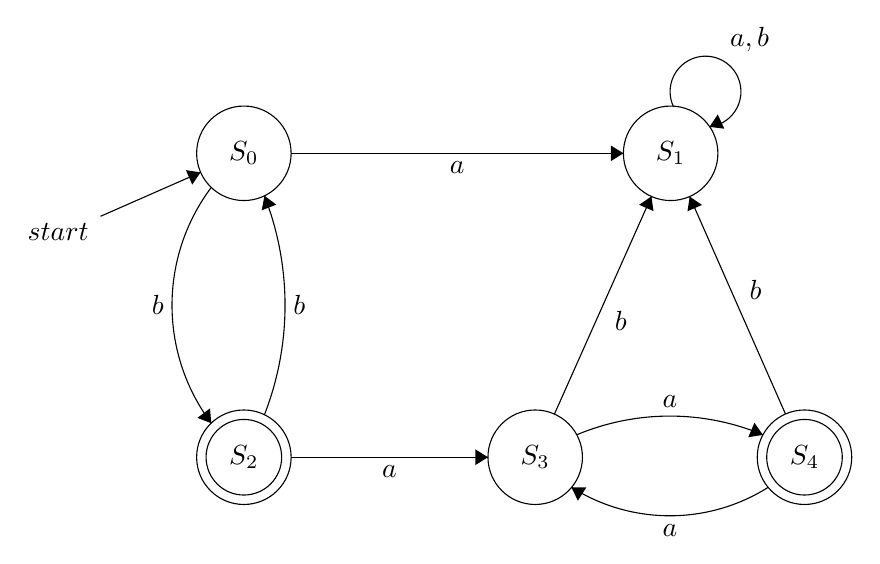
\begin{tikzpicture}[scale=0.2]
\tikzstyle{every node}+=[inner sep=0pt]
\draw [black] (23.2,-15.6) circle (3);
\draw (23.2,-15.6) node {$S_0$};
\draw [black] (50.3,-15.6) circle (3);
\draw (50.3,-15.6) node {$S_1$};
\draw [black] (23.2,-34.9) circle (3);
\draw (23.2,-34.9) node {$S_2$};
\draw [black] (23.2,-34.9) circle (2.4);
\draw [black] (41.7,-34.9) circle (3);
\draw (41.7,-34.9) node {$S_3$};
\draw [black] (58.8,-34.9) circle (3);
\draw (58.8,-34.9) node {$S_4$};
\draw [black] (58.8,-34.9) circle (2.4);
\draw [black] (14.1,-19.6) -- (20.45,-16.81);
\draw (13.37,-20.58) node [left] {$start$};
\fill [black] (20.45,-16.81) -- (19.52,-16.67) -- (19.92,-17.59);
\draw [black] (26.2,-15.6) -- (47.3,-15.6);
\fill [black] (47.3,-15.6) -- (46.5,-15.1) -- (46.5,-16.1);
\draw (36.75,-16.1) node [below] {$a$};
\draw [black] (50.468,-12.616) arc (204.51457:-83.48543:2.25);
\draw (55.31,-9.22) node [above] {$a,b$};
\fill [black] (52.77,-13.92) -- (53.71,-14.04) -- (53.29,-13.13);
\draw [black] (21.131,-32.738) arc (-143.1429:-216.8571:12.483);
\fill [black] (21.13,-32.74) -- (21.05,-31.8) -- (20.25,-32.4);
\draw (18.14,-25.25) node [left] {$b$};
\draw [black] (24.505,-18.298) arc (21.32678:-21.32678:19.116);
\fill [black] (24.51,-18.3) -- (24.33,-19.22) -- (25.26,-18.86);
\draw (26.31,-25.25) node [right] {$b$};
\draw [black] (26.2,-34.9) -- (38.7,-34.9);
\fill [black] (38.7,-34.9) -- (37.9,-34.4) -- (37.9,-35.4);
\draw (32.45,-35.4) node [below] {$a$};
\draw [black] (44.335,-33.476) arc (112.75847:67.24153:15.29);
\fill [black] (56.16,-33.48) -- (55.62,-32.71) -- (55.23,-33.63);
\draw (50.25,-31.79) node [above] {$a$};
\draw [black] (56.496,-36.809) arc (-57.70157:-122.29843:11.69);
\fill [black] (44,-36.81) -- (44.41,-37.66) -- (44.95,-36.81);
\draw (50.25,-39.12) node [below] {$a$};
\draw [black] (42.92,-32.16) -- (49.08,-18.34);
\fill [black] (49.08,-18.34) -- (48.3,-18.87) -- (49.21,-19.27);
\draw (46.73,-26.24) node [right] {$b$};
\draw [black] (57.59,-32.15) -- (51.51,-18.35);
\fill [black] (51.51,-18.35) -- (51.37,-19.28) -- (52.29,-18.88);
\draw (55.28,-24.27) node [right] {$b$};
\end{tikzpicture}
\end{center}

\subsection*{Question (b):}
$$b\bigg(bb\bigg)^{*}\bigg(aa\bigg)^*$$
















\newpage
\section*{Question 5:}
Consider the language $L = \{a^n\ b^m|n  \neq m\}$; as we have seen this is not regular. Recall the definition of the equivalence $\equiv_L$ which we used in the proof of the Myhill-Nerode theorem. Since this language is not regular $\equiv_L$ cannot have finitely many equivalence classes. Exhibit explicitly, infinitely many distinct equivalence classes of $\equiv_L$.\\
\newline
\newline
Given any language $L \subseteq \Sigma^*$, not necessarily regular, we define an equivalence relation $R_L$ on $\Sigma^*$ as follows
$$x\ R_L\ y \text{ if and only if } \forall z, xz \in L \Leftrightarrow yz \in L$$.
\\ \newline
We just need to construct infinite many equivalence relation $R_L$:\\
To begin with, I choose $x = a^{k_1} \quad y = a^{k_2} \quad k_1 \neq k_2 \quad k_1, k_2 \in \mathbb{N}$\\
Then obviously, we have infinite many pairs of such $x, y$.\\
Then we choose $z = b^{k_1}$, thus, we have $xz \notin L \quad yz \in L$, which means $x, y$ not in equivalence relationship.\\
As there are infinite pairs of such $x, y$, we can say: infinitely many distinct equivalence classes of $R_L$.\\






























\end{document}